



\newpage
\section{Excited states}
\label{sec:ES}

%We shall now examine the case of a square lattice with boundary conditions, i.e. the toric code. \newline

Taking into account the results yielded by the examination of the physical system in the previous chapters we will now proceed to describe, firstly, what are the excitations on the ground state and what kind of excitations we can obtain on the ground state; after this, we will examine the exchange statistics of the excitations.\newline
In general, the low-energy excitations of a quantum system, often referred to as quasiparticles, represent deviations from the system's ground state. These excitations are associated with elementary quantum particles that can be created or annihilated with relatively low energy. The properties of these quasiparticles, including their statistics, are crucial for gaining insights into the system's ground state degeneracy, topological properties, and response to external perturbations. \newline

In the particular case of the Toric Code, such low-energy excitations can be created in two ways: 

\begin{enumerate}
	\item through the application of an open-ended string $S^x$ made up of $\sigma^x$ operators on the ground state;
	
	\item through the application of an open-ended string $S^z$ made up of $\sigma^z$ operators on the ground state.
\end{enumerate}

At the extremities of the above mentioned strings, particles are created. We will call the pairs of particles obtained through the application of operator $S^x$ \textit{electric charges}, while the ones obatained by applying an $S^z$ operator to the ground states \textit{magnetic vortices}.\newline

%picture
\begin{figure}[b]
	
	\begin{center}
		
		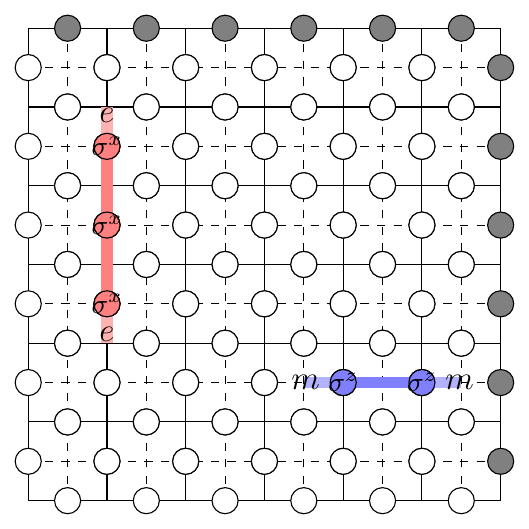
\begin{tikzpicture}
			% Draw dashed lines
			\foreach \i in {-3,-2.5,...,3}
			{
				\draw[dashed] (\i,-3) -- (\i,3);
			}
			\foreach \j in {-3,-2.5,...,3}
			{
				\draw[dashed] (-3,\j) -- (3,\j);
			}
			
			
			
			% Draw solid grid and nodes with circles in the middle of each side
			\draw[step=1cm] (-3,-3) grid (3,3);
			\foreach \i in {-2.5,...,2.5}
			{
				\foreach \j in {-2.5,...,2.5}
				{
					
					
					\begin{scope}[transform canvas={xshift=\i cm,yshift=\j cm}]
						\node[right,xshift=0.2cm,yshift=0.4cm] {};
						% Convert \j and \i to integers
						\pgfmathtruncatemacro{\intj}{\j}
						\pgfmathtruncatemacro{\inti}{\i}
						
						% Draw circles at the midpoints of each side
						\ifnum\intj=2
						\draw node[draw,circle,fill=gray] at (0,0.5) {};
						\else
						\draw node[draw,circle,fill=white] at (0,0.5) {};
						\fi
						
						\ifnum\inti=2
						\draw node[draw,circle,fill=gray] at (0.5,0) {};
						\else
						\draw node[draw,circle,fill=white] at (0.5,0) {};
						\fi
						
						\draw node[draw,circle,fill=white] at (0,-0.5) {};
						\draw node[draw,circle,fill=white] at (-0.5,0) {};
					\end{scope}
				}
			}
			
			\foreach \i in {-2,...,-2}
			{
				\draw[red!30, line width=1.5mm] (\i,-1) -- (\i,-0.5);
				\draw[red!50, line width=1.5mm] (\i,-0.5) -- (\i,1.5);
				\draw[red!30, line width=1.5mm] (\i,1.5) -- (\i,2);
				\node[draw, circle, fill=red!50,label=center:\textbf{$\sigma^x$},label=south:\textbf{\large \bf $e$}] at (\i,-0.5) {};
				\node[draw, circle, fill=red!50,label=center:\textbf{$\sigma^x$}] at (\i,0.5) {};
				\node[draw, circle, fill=red!50,label=center:\textbf{$\sigma^x$},label=north:\textbf{\bf \large $e$}] at (\i,1.5) {};
				
			}
			
			\foreach \j in {-1.5,...,-1.5}
			{
				\draw[blue!30, line width=1.5mm] (0.5, \j) -- (1, \j);
				\draw[blue!50, line width=1.5mm] (1, \j) -- (2, \j);
				\draw[blue!30, line width=1.5mm] (2, \j) -- (2.5, \j);
				
				\draw node[draw,circle,fill=blue!50,label=center:\textbf{$\sigma^z$},label=left:\textbf{\large \bf $m$}] at (1,\j) {};
				\draw node[draw,circle,fill=blue!50,label=center:\textbf{$\sigma^z$},label=right:\textbf{\large \bf $m$}] at (2,\j) {};
				
			}
			
			
		\end{tikzpicture}
	\end{center}
	
	\caption{$e$ and $m$ excitations on the ground state.}
	\label{fig:excitations}
\end{figure}





\newpage
We can prove that if a string $S^x$ of $\sigma^x$ operators is open-ended, then the $\sigma^x$ operators at its two extremes of the string will anticommute with one $A_v$ each. \newline 

\textit{Proof.}\newline
We want to show that $A_v S^x + S^x A_v=0$.\newline

Knowing that 

\begin{center}
	$A_v = \prod_{i=1}^{4} \sigma_i^z$ \\ 
	$S^x = \prod_{j=1}^{N} \sigma_j^x$
\end{center}

by substitution we obtain the following expression: \newline

\begin{center}
	$\prod_{i=1}^{4} \prod_{j=1}^{N} \sigma_j^x + \prod_{j=1}^{N} \sigma_j^x \prod_{i=1}^{4} \sigma_i^z = 0$ $(1)$
\end{center}

remeber that only one $\sigma_i^z$ will overlap with the extremity of the string $S^x$; thus, only one $\sigma_i^z$ will anticommute with the extremity of the string $S^x$. Knowing that for Pauli matrices acting on the same edge we have anticommutation

\begin{center}
	$\sigma_{v'}^x \sigma_{v'}^z = - \sigma_{v'}^z \sigma_v^x$ for $v=v'$ \\
	$\sigma_v^x \sigma_{v'}^z =  \sigma_{v'}^z \sigma_v^x$ for $v \neq v'$ 
\end{center}

if for simplicity we fix $N=2$ we can easily see that :\newline

\begin{center}
	$(\sigma_1^z \sigma_2^z \sigma_3^z \sigma_4^z)(\sigma_1^x \sigma_2^x)  = - (\sigma_1^x \sigma_2^x)(\sigma_1^z \sigma_2^z \sigma_3^z \sigma_4^z) $ 
\end{center}

having supposed that, for example, the extremity $\sigma_1^x$ overlaps with the $\sigma_3^z$ edge part of the $A_v$ operator. This can then be easily generalized for $N$ Pauli operators. Finally, if we substitute such expressione in $(1)$ we obtain that the overall equation is in fact equal to zero.\newline

This procedure should be iterated also for the other extremity of the string $S^x$ to show that the operator commutes with two $A_v$ operators, one for each endpoint.\newline

\hfill $\square$ \newline

In the same way, we could prove that, if we take a string $S^z$ made up of $\sigma_z$ operators still open-ended, the $\sigma^z$ operators at its endpoints will anticommute with one $B_p$ each.\newline


The effect of putting such strings on the ground states correspond to raising the associated energy of the GS by 2. In fact, coherently with what said in \textit{\cite{Her20}}, it is impossible to create unitary excitations on the ground states.

\begin{proposition}(Magnitude of the excitations)
	Placing string operators on the ground states correspond to raising the associated energy of the GS by 2.
\end{proposition}

\textit{Proof.} \newline
Recall that for a string operator, here we will choose $S^x$, both equations hold:

\begin{center}
	$\begin{cases} 
		A_{v1} S^x + S^x A_{v1} =0 \\
		A_{v2} S^x + S^x A_{v2} =0
	\end{cases}$ 
\end{center}

If we apply the string operator to the Ground State, taking into account anticommutativity stated above, we obtain that:

\begin{center}
	$\begin{cases}
		A_{v1} S^x |GS\rangle = - S^x A_{v1} |GS\rangle = - S^x |GS\rangle \\
		
		A_{v2} S^x |GS\rangle = - S^x A_{v2} |GS\rangle = - S^x |GS\rangle
	\end{cases}$ 
\end{center}

since $A_{v1}|GS\rangle = +1|GS\rangle$ and $A_{v2}|GS\rangle = +1|GS\rangle$.
Summing up term by term :

\begin{center}
	$\begin{cases}
		A_{v1} S^x |GS\rangle + A_{v2} S^x |GS\rangle = - 2 S^x A_{v1} |GS\rangle
	\end{cases}$ 
\end{center}

Thus, if the energy of the Ground State as we have defined it in the previous chapters is $-2N$ by acting with a string operator on  it we obtain a final energy equal to $-2N+2$.

\hfill $\square$ \newline

%Firstly, we study the individual statistics of electric charges and magnetic votices, then we argue their mutual statistics.\newline

Let's analyze the statistics of $e$-particles in the context of the ground state. If we take a simple string operator $\sigma^z|GS\rangle$ , where $|GS\rangle$ denotes the ground state, it creates two e-particles in the vertices adjacent to the edge as shown in figure 1.11. \newline 
We know that a string operator of the form $\prod_{j=1}^{N} \sigma_j^z$ allows the separation of these two excitations. In fact, as illustrated below, the exchange of these particles becomes possible by applying the string operator in such a way that it moves the excitations around the lattice until they reach configuration shown in figure 1.11(c). 
However, due to the commutation of all $\sigma^x$ with each other, after the application of a closed loop of $\sigma^x$ (last passage in figure 1.11), there is no overall acquired phase. Consequently, the $e$-excitations exhibit bosonic statistics. A similar argument can be made for the $m$-excitations, establishing them as bosons as well.\newline

%picture
\begin{figure}
\begin{center}
	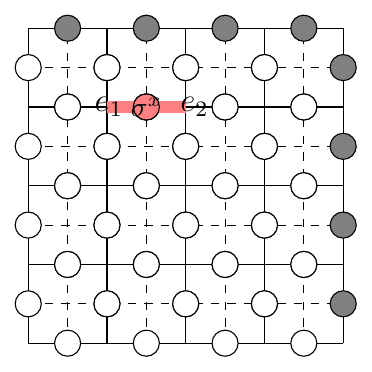
\begin{tikzpicture}
		% Draw dashed lines
		\foreach \i in {-2,-1.5,...,2}
		{
			\draw[dashed] (\i,-2) -- (\i,2);
		}
		\foreach \j in {-2,-1.5,...,2}
		{
			\draw[dashed] (-2,\j) -- (2,\j);
		}
		
		
		% Draw solid grid and nodes with circles in the middle of each side
		\draw[step=1cm] (-2,-2) grid (2,2);
		\foreach \i in {-1.5,...,1.5}
		{
			\foreach \j in {-1.5,...,1.5}
			{
				\begin{scope}[transform canvas={xshift=\i cm,yshift=\j cm}]
					\node[right,xshift=0.2cm,yshift=0.4cm] {};
					% Convert \j and \i to integers
					\pgfmathtruncatemacro{\intj}{\j}
					\pgfmathtruncatemacro{\inti}{\i}
					
					% Draw circles at the midpoints of each side
					\ifnum\intj=1
					\draw node[draw,circle,fill=gray] at (0,0.5) {};
					\else
					\draw node[draw,circle,fill=white] at (0,0.5) {};
					\fi
					
					\ifnum\inti=1
					\draw node[draw,circle,fill=gray] at (0.5,0) {};
					\else
					\draw node[draw,circle,fill=white] at (0.5,0) {};
					\fi
					
					\draw node[draw,circle,fill=white] at (0,-0.5) {};
					\draw node[draw,circle,fill=white] at (-0.5,0) {};
				\end{scope}
			}
		}
		
		
		
		
		\foreach \j in {1,...,1}
		{
			
			\draw[red!50, line width=1.5mm] (-1, \j) -- (-0.5, \j);
			%\draw node[label=north:\textbf{ \large $e_1$}] at (-1,\j) {};
			\draw[red!50, line width=1.5mm] (-0.5, \j) -- (0, \j);
			%\draw node[label=north:\textbf{ \large $e_2$}] at (0,\j) {};
			\node[draw, circle, fill=red!50,label=center:\textbf{$\sigma^x$},label=left:\textbf{ \large $e_1$},label=right:\textbf{ \large $e_2$}] at (-0.5,1) {};
			
		}
		
	\end{tikzpicture}
\end{center}

\vspace*{1cm}

\begin{center}
	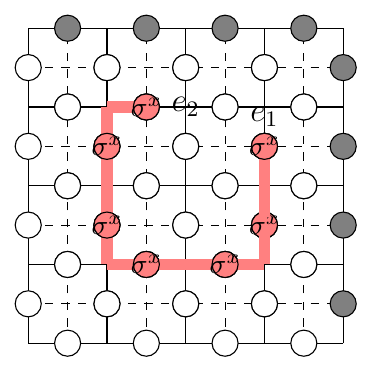
\begin{tikzpicture}
		% Draw dashed lines
		\foreach \i in {-2,-1.5,...,2}
		{
			\draw[dashed] (\i,-2) -- (\i,2);
		}
		\foreach \j in {-2,-1.5,...,2}
		{
			\draw[dashed] (-2,\j) -- (2,\j);
		}
		
		
		% Draw solid grid and nodes with circles in the middle of each side
		\draw[step=1cm] (-2,-2) grid (2,2);
		\foreach \i in {-1.5,...,1.5}
		{
			\foreach \j in {-1.5,...,1.5}
			{
				\begin{scope}[transform canvas={xshift=\i cm,yshift=\j cm}]
					\node[right,xshift=0.2cm,yshift=0.4cm] {};
					% Convert \j and \i to integers
					\pgfmathtruncatemacro{\intj}{\j}
					\pgfmathtruncatemacro{\inti}{\i}
					
					% Draw circles at the midpoints of each side
					\ifnum\intj=1
					\draw node[draw,circle,fill=gray] at (0,0.5) {};
					\else
					\draw node[draw,circle,fill=white] at (0,0.5) {};
					\fi
					
					\ifnum\inti=1
					\draw node[draw,circle,fill=gray] at (0.5,0) {};
					\else
					\draw node[draw,circle,fill=white] at (0.5,0) {};
					\fi
					
					\draw node[draw,circle,fill=white] at (0,-0.5) {};
					\draw node[draw,circle,fill=white] at (-0.5,0) {};
				\end{scope}
			}
		}
		
		
		
		
		\foreach \j in {1,...,1}
		{
			
			\draw[red!50, line width=1.5mm] (-1, \j) -- (-0.5, \j);
			\draw node[label=center:\textbf{\large $e_2$}] at (0,\j) {};
			%\draw[red!50, line width=1.5mm] (-0.5, \j) -- (0, \j);
			
			\node[draw, circle, fill=red!50,label=center:\textbf{$\sigma^x$}] at (-0.5,1) {};
			
		}
		
		\foreach \i in {-1,...,-1}
		{
			
			\draw[red!50, line width=1.5mm] (\i,1) -- (\i,-1);
			%\draw node[label=north:\textbf{e1}] at (\i,0) {};
			%\draw[blue!50, line width=1.5mm] (\i,0) -- (\i,0);
			
			\node[draw, circle, fill=red!50,,label=center:\textbf{$\sigma^x$}] at (-1,0.5) {};
			\node[draw, circle, fill=red!50,,label=center:\textbf{$\sigma^x$}] at (-1,-0.5) {};
			
		}
		
		\foreach \j in {-1,...,-1}
		{
			
			\draw[red!50, line width=1.5mm] (-1, \j) -- (1, \j);
			
			
			\node[draw, circle, fill=red!50,label=center:\textbf{$\sigma^x$}] at (0.5,-1) {};
			\node[draw, circle, fill=red!50,label=center:\textbf{$\sigma^x$}] at (1,-0.5) {};
			\node[draw, circle, fill=red!50,label=center:\textbf{$\sigma^x$}] at (-0.5,-1) {};
			
		}
		
		\foreach \i in {1,...,1}
		{
			
			\draw[red!50, line width=1.5mm] (\i,-0.4) -- (\i,0.4);
			\draw node[label=north:\textbf{\large $e_1$}] at (\i,0.5) {};
			%\draw[blue!50, line width=1.5mm] (\i,0) -- (\i,0);
			\draw[red!50, line width=1.5mm] (\i,-1) -- (\i,-0.6);
			
			\node[draw, circle, fill=red!50,,label=center:\textbf{$\sigma^x$}] at (1,0.5) {};
			
		}
		
		
		
	\end{tikzpicture}
\end{center}

\vspace*{1cm}

\begin{center}
	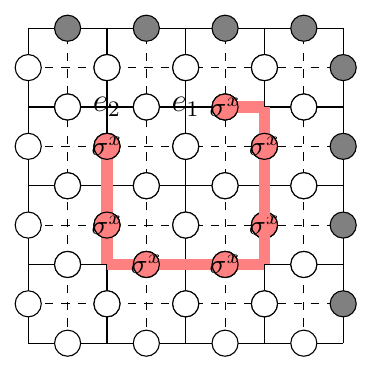
\begin{tikzpicture}
		% Draw dashed lines
		\foreach \i in {-2,-1.5,...,2}
		{
			\draw[dashed] (\i,-2) -- (\i,2);
		}
		\foreach \j in {-2,-1.5,...,2}
		{
			\draw[dashed] (-2,\j) -- (2,\j);
		}
		
		
		% Draw solid grid and nodes with circles in the middle of each side
		\draw[step=1cm] (-2,-2) grid (2,2);
		\foreach \i in {-1.5,...,1.5}
		{
			\foreach \j in {-1.5,...,1.5}
			{
				\begin{scope}[transform canvas={xshift=\i cm,yshift=\j cm}]
					\node[right,xshift=0.2cm,yshift=0.4cm] {};
					% Convert \j and \i to integers
					\pgfmathtruncatemacro{\intj}{\j}
					\pgfmathtruncatemacro{\inti}{\i}
					
					% Draw circles at the midpoints of each side
					\ifnum\intj=1
					\draw node[draw,circle,fill=gray] at (0,0.5) {};
					\else
					\draw node[draw,circle,fill=white] at (0,0.5) {};
					\fi
					
					\ifnum\inti=1
					\draw node[draw,circle,fill=gray] at (0.5,0) {};
					\else
					\draw node[draw,circle,fill=white] at (0.5,0) {};
					\fi
					
					\draw node[draw,circle,fill=white] at (0,-0.5) {};
					\draw node[draw,circle,fill=white] at (-0.5,0) {};
				\end{scope}
			}
		}
		
		
		
		
		\foreach \j in {1,...,1}
		{
			
			\draw[red!50, line width=1.5mm] (0.5, \j) -- (1, \j);
			\draw node[label=center:\textbf{\large $e_1$}] at (0,\j) {};
			\draw node[draw, circle, fill=red!50,label=center:\textbf{$\sigma^x$}] at (0.5,\j) {};
			%\draw node[label=center:\textbf{e2}] at (0,\j) {};
			%\draw[red!50, line width=1.5mm] (-0.5, \j) -- (0, \j);
			
			%\node[draw, circle, fill=red!50,label=center:\textbf{$\sigma^x$}] at (-0.5,1) {};
			
		}
		
		\foreach \i in {-1,...,-1}
		{
			
			\draw[red!50, line width=1.5mm] (\i,-1) -- (\i,0.5);
			\draw node[label=center:\textbf{\large $e_2$}] at (\i,1) {};
			
			\node[draw, circle, fill=red!50,label=center:\textbf{$\sigma^x$}] at (-1,0.5) {};
			\node[draw, circle, fill=red!50,label=center:\textbf{$\sigma^x$}] at (-1,-0.5) {};
			
		}
		
		\foreach \j in {-1,...,-1}
		{
			
			\draw[red!50, line width=1.5mm] (-1, \j) -- (1, \j);
			
			
			\node[draw, circle, fill=red!50,label=center:\textbf{$\sigma^x$}] at (0.5,-1) {};
			\node[draw, circle, fill=red!50,label=center:\textbf{$\sigma^x$}] at (1,-0.5) {};
			\node[draw, circle, fill=red!50,label=center:\textbf{$\sigma^x$}] at (-0.5,-1) {};
			
		}
		
		\foreach \i in {1,...,1}
		{
			
			\draw[red!50, line width=1.5mm] (\i,-0.4) -- (\i,0.4);
			\draw[red!50, line width=1.5mm] (\i,-1) -- (\i,-0.6);
			\draw[red!50, line width=1.5mm] (\i,0.6) -- (\i,1);
			
			\node[draw, circle, fill=red!50,,label=center:\textbf{$\sigma^x$}] at (1,0.5) {};
			
		}
		
		
		
	\end{tikzpicture}
\end{center}

\vspace*{1cm}

\begin{center}
	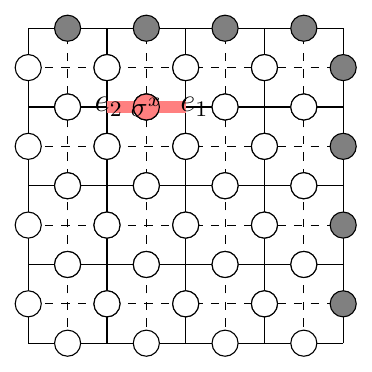
\begin{tikzpicture}
		% Draw dashed lines
		\foreach \i in {-2,-1.5,...,2}
		{
			\draw[dashed] (\i,-2) -- (\i,2);
		}
		\foreach \j in {-2,-1.5,...,2}
		{
			\draw[dashed] (-2,\j) -- (2,\j);
		}
		
		
		% Draw solid grid and nodes with circles in the middle of each side
		\draw[step=1cm] (-2,-2) grid (2,2);
		\foreach \i in {-1.5,...,1.5}
		{
			\foreach \j in {-1.5,...,1.5}
			{
				\begin{scope}[transform canvas={xshift=\i cm,yshift=\j cm}]
					\node[right,xshift=0.2cm,yshift=0.4cm] {};
					% Convert \j and \i to integers
					\pgfmathtruncatemacro{\intj}{\j}
					\pgfmathtruncatemacro{\inti}{\i}
					
					% Draw circles at the midpoints of each side
					\ifnum\intj=1
					\draw node[draw,circle,fill=gray] at (0,0.5) {};
					\else
					\draw node[draw,circle,fill=white] at (0,0.5) {};
					\fi
					
					\ifnum\inti=1
					\draw node[draw,circle,fill=gray] at (0.5,0) {};
					\else
					\draw node[draw,circle,fill=white] at (0.5,0) {};
					\fi
					
					\draw node[draw,circle,fill=white] at (0,-0.5) {};
					\draw node[draw,circle,fill=white] at (-0.5,0) {};
				\end{scope}
			}
		}
		
		
		
		
		\foreach \j in {1,...,1}
		{
			
			\draw[red!50, line width=1.5mm] (-1, \j) -- (-0.5, \j);
			%\draw node[label=north:\textbf{ \large $e_1$}] at (-1,\j) {};
			\draw[red!50, line width=1.5mm] (-0.5, \j) -- (0, \j);
			%\draw node[label=north:\textbf{ \large $e_2$}] at (0,\j) {};
			\node[draw, circle, fill=red!50,label=center:\textbf{$\sigma^x$},label=left:\textbf{ \large $e_2$},label=right:\textbf{ \large $e_1$}] at (-0.5,1) {};
			
		}
		
	\end{tikzpicture}
\end{center}


\caption{In the first picture we show the creation of a pair of $e$-excitations on the ground state by means of $\sigma^x$ operator. In the following pictures we move around the excitations using a string operator until we reach the configuration in the third picture. In the last passage we apply a closed loop of $\sigma^x$ in order to go back to the first kind of configuartion. }
\label{fig:base}
\end{figure}

%--------------------------






